\documentclass[german]{beamer}

\mode<presentation>
{
  \usetheme{Warsaw}
  \setbeamercovered{transparent}
}

\usepackage{latexsym}
\usepackage{url}
\usepackage{appendixnumberbeamer}

%\usepackage{german}
\usepackage[latin1]{inputenc} %% Umlaute

\usepackage{stmaryrd,mathbbol,mathrsfs}
\usepackage{amsmath,amstext,amssymb,amsopn}
\usepackage{exscale,calc,ifthen,array}
\usepackage{float}
\usepackage{overpic}


\usepackage{xspace,alltt}
\usepackage{amssymb}
\usepackage[ps,dvips]{xy}
\xyoption{v2}
\xyoption{line}
\xyoption{curve}

%\definecolor{red}{rgb}{1,0,0} % red
%\definecolor{green}{rgb}{0,1,0} % green
%\definecolor{blue}{rgb}{0,0,1} % blue

\newcommand{\emphc}[1]{{\color{red}{#1}}}

\newcommand{\red}[1]{{\color{red}{#1}}}
\newcommand{\green}[1]{{\color{green}{#1}}}
\newcommand{\blue}[1]{{\color{blue}{#1}}}
\newcommand{\white}[1]{{\color{white}{#1}}}


\newlength{\PicSize}
\newcommand{\CASL}{\textsc{CASL}\xspace}
\newcommand{\HetCASL}{\textmd{\textsc{HetCasl}}\xspace }
\newcommand{\Hets}{\textmd{\textsc{Hets}}\xspace }

\newcommand{\mystrut}[1]{\rule[#1]{0cm}{0.1cm}}


%% Note: If title has linebreaks, you must use a short title without 
%%       linebreaks, otherwise you'll get funny LaTeX errors.
\title{OntoHub Perspectives}

%% Note about linebreaks applies here as well.
\author{The Ontohub team}

\date{12.12.12}

\logo{
\includegraphics[height=0.8cm]{DFKI-Logo.jpg}
\hspace{5.5cm}

\includegraphics[height=0.8cm]{sfb_tr8_logo.pdf}}

\begin{document}

\maketitle

\begin{frame}
\frametitle{Time plan}
\begin{tabular}{|l|p{9cm}|}\hline
10h & Intro / Motivation / Know-How\\\hline
10.30h & Ontohub and its background (OntoIOp ISO standard, OOR community, Hets community)\\\hline
11h & Ontohub.org web portal demo\\\hline
11.30h & Ontohub architecture and data model\\\hline
13h & Lunch\\\hline
14h & Aims\\\hline
14.30h & Motivation / Know-How / Work areas\\\hline
15h & Organisation (regular meetings, programming sessions, github, issue tracker)\\\hline
15.30h & Setup of development environment\\\hline
ca. 16h & End\\\hline
\end{tabular}
\end{frame}

\begin{frame}
\frametitle{External advice}
Michael Gruninger, Toronto

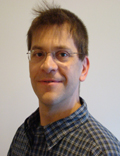
\includegraphics[width=0.5\textwidth]{MGpic.jpg}
\end{frame}

\begin{frame}
\frametitle{Ontologies}
\begin{itemize}
\item Ontology = shared (formal) conceptualisation (of a domain)
\item Example: Pizza ontology 
\begin{itemize}
\item using Web Ontology Language OWL
\item tool for editing OWL ontologies: Prot�g� \url{http://protege.stanford.edu/}
\end{itemize}
\end{itemize}
\end{frame}

\begin{frame}
\frametitle{Applications of Ontologies}
\begin{itemize}
\item Medicine (Snomed)
\item Biology, Biochemistry (molecules \ldots)
\item Semantic Web
\begin{itemize}
\item Semantic Mediawiki
\begin{itemize}
\item better categories for Wikipedia
\end{itemize}
\item schema.org (Google, Yahoo, Microsoft)
\begin{itemize}
\item structured content for HTML pages
\end{itemize}
\end{itemize}
\end{itemize}
\end{frame}

\begin{frame}
\frametitle{Open Ontology Repository (OOR)}
\begin{itemize}
\item ambitious goals:
\begin{itemize}
\item establishing a hosted registry-repository;
\item enabling and facilitating open, federated, collaborative ontology repositories, and
\item establishing best practices for expressing interoperable ontology and taxonomy work in registry-repositories.
\end{itemize}
\item lots of OOR presentations at conferences
\item regular Skype conferences
\item implementation: only through Bioportal, only for OWL
\item \url{http://www.oor.net}
\end{itemize}
\end{frame}

\begin{frame}
\frametitle{BioPortal}
\vspace{-1cm}
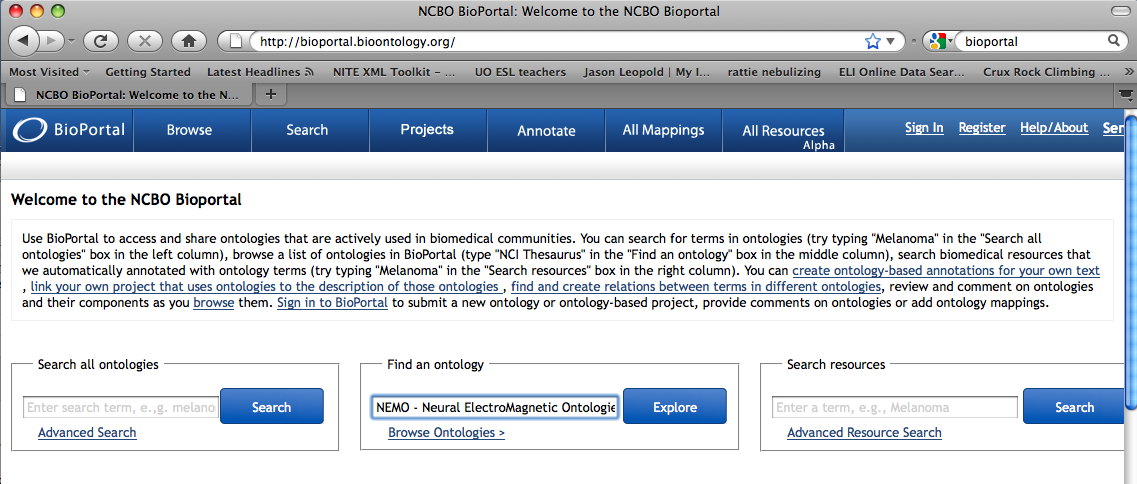
\includegraphics[width=1\textwidth]{Screenshot_Bioportal.png}
\end{frame}

\begin{frame}
\frametitle{Ontology Integration and Interoperability (OntoIOp)}
\begin{itemize}
\item ISO Standard 17347 (currently: working draft)
\item Distributed Ontology Language (DOL)
\begin{itemize}
\item OWL (Web Ontology Language)
\item RDF (Resource Description Framework)
\item EER (Enhanced Entity-Relationship Diagrams)
\item Common Logic
\item UML (Unified Modeling Language)
\item \ldots
\end{itemize}
\item Community of 10-15 experts
\item bi-weekly Skype conferences
\item \url{http://ontoiop.org}
\end{itemize}
\end{frame}

\begin{frame}
\frametitle{OntoIOp Logic Graph}
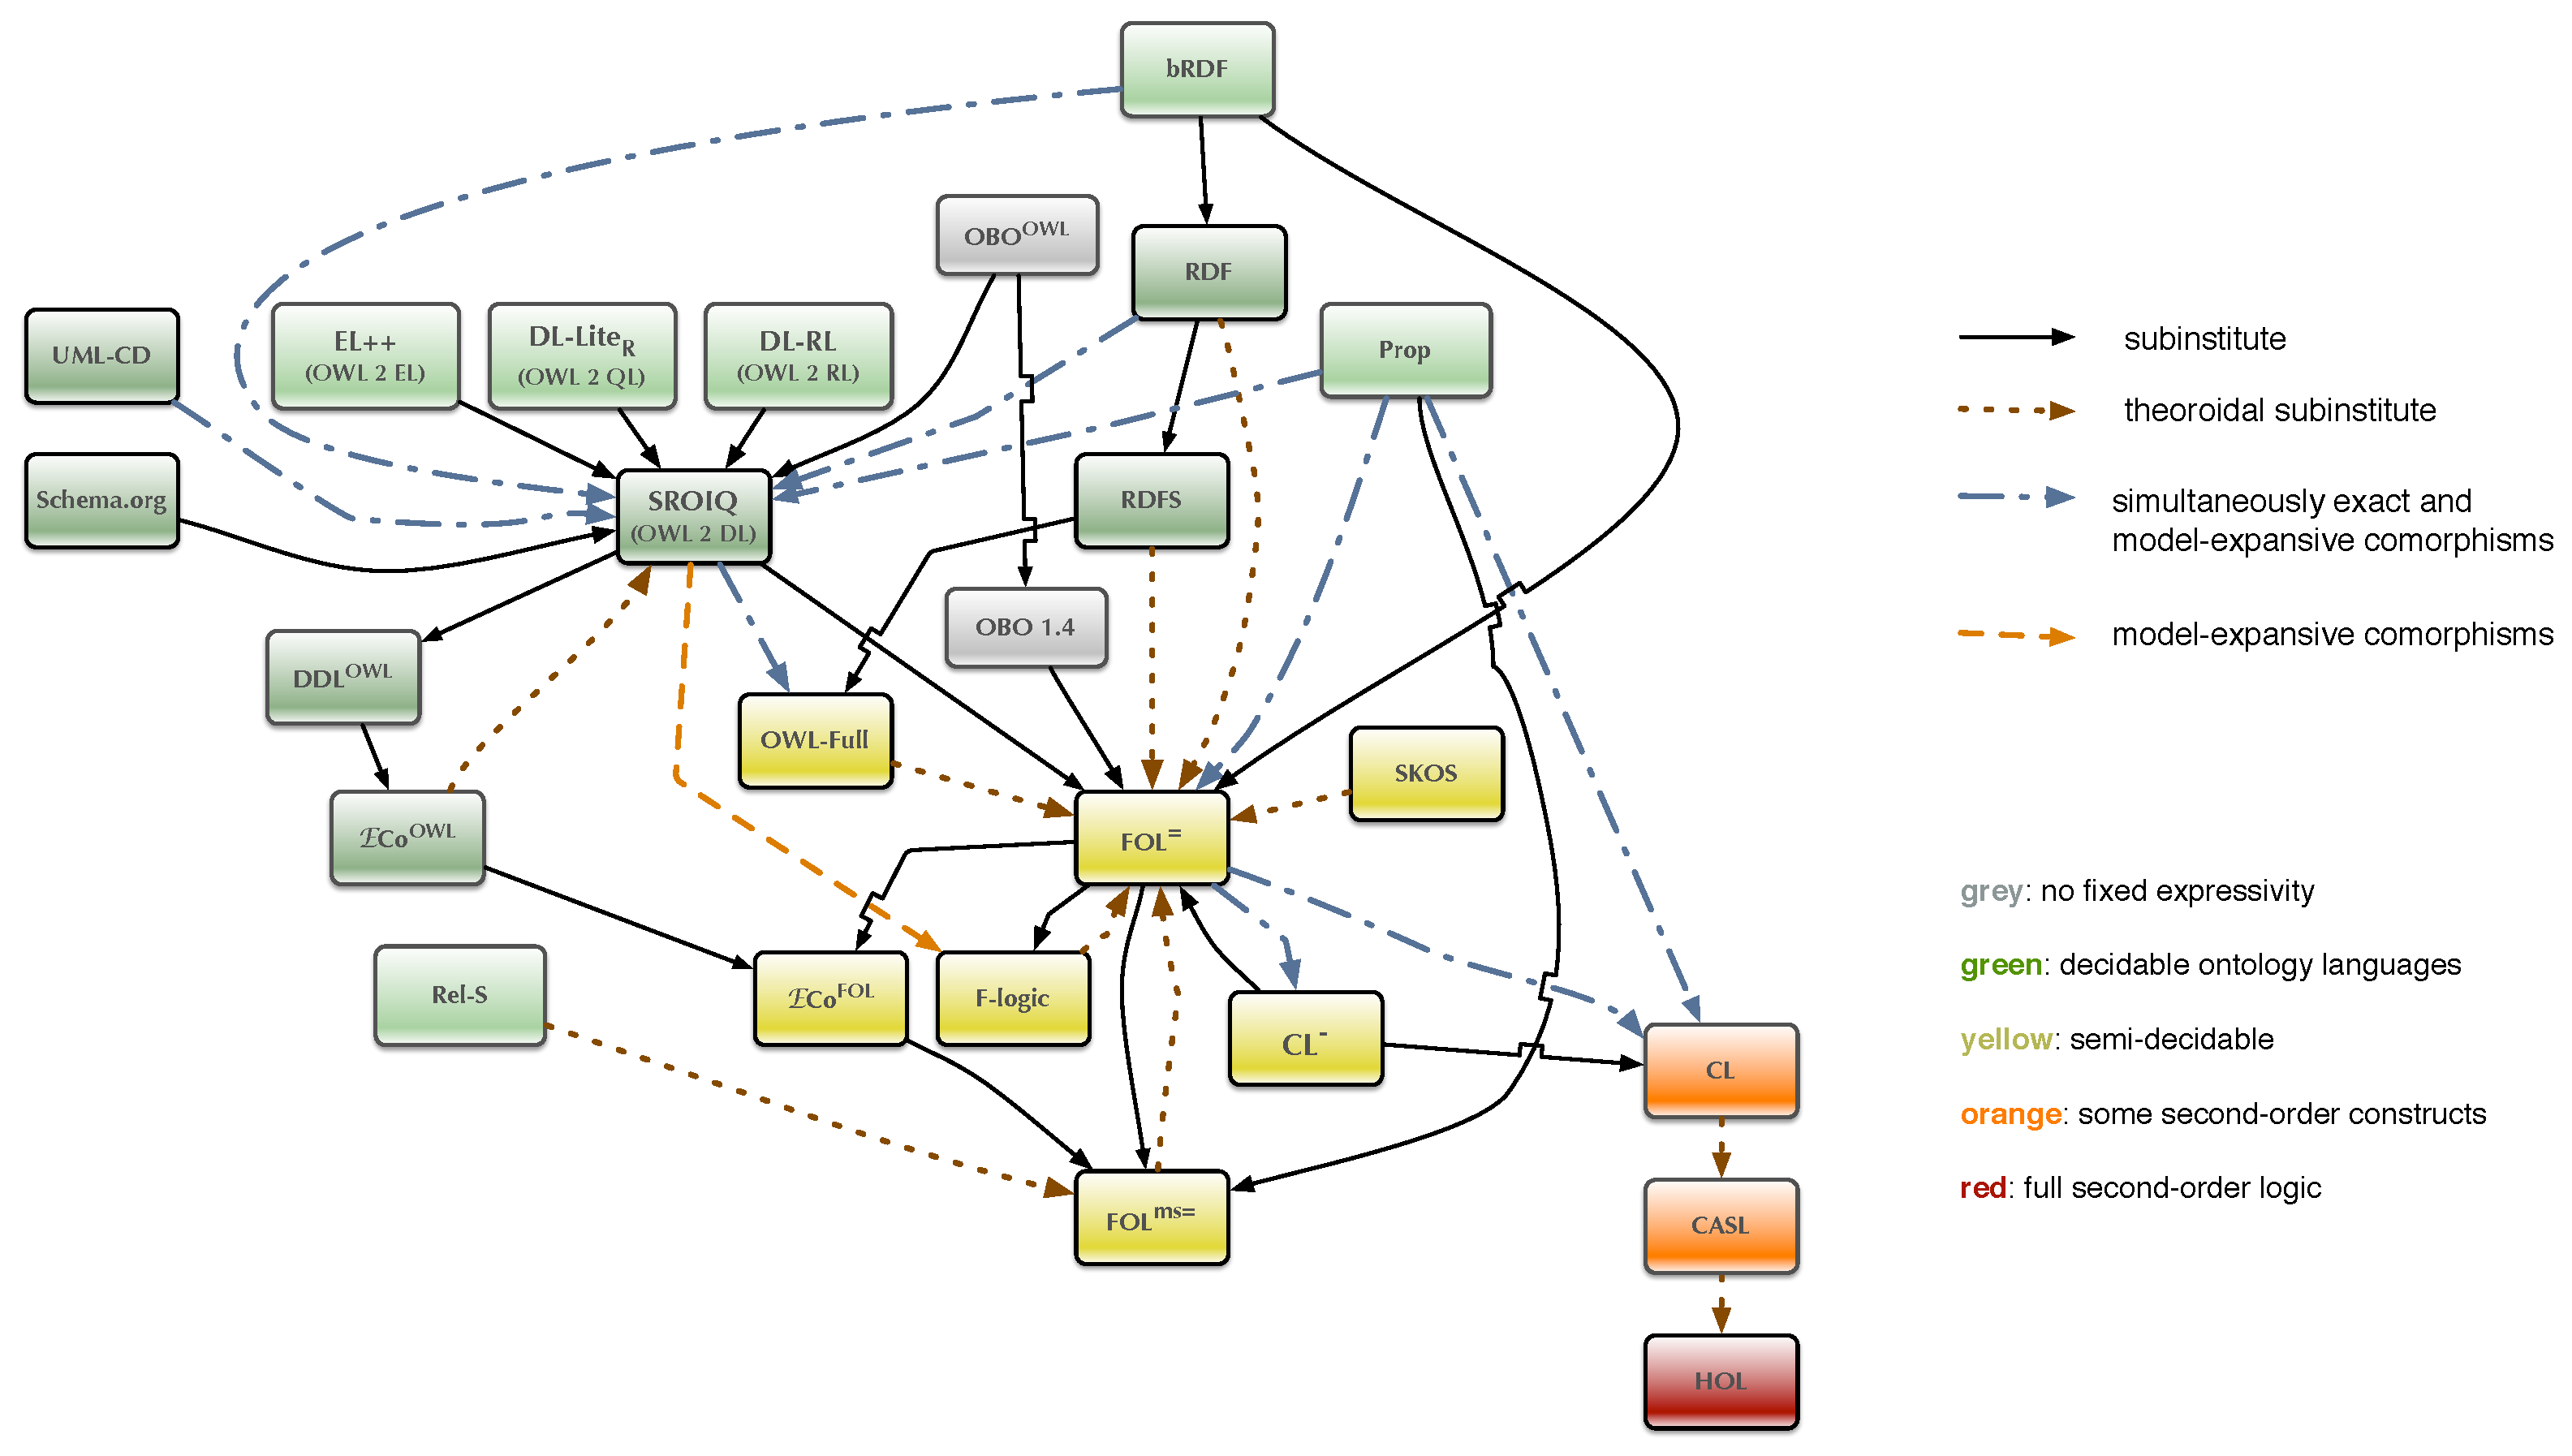
\includegraphics[width=\textwidth]{ontograph}
\end{frame}

\begin{frame}
\frametitle{Heterogeneous Tool Set (Hets)}
\begin{itemize}
\item Logic backend for OntoHub
\item can parse and analyse all involved languages
\item implements logic translations
\item interface to about 15 proof tools
\item anchored in algebraic specification community\\ (WADT, CoFI, IFIP WG 1.3) 
\item \url{http://www.dfki.de/cps/hets}
\end{itemize}
\end{frame}


\begin{frame}
\frametitle{OntoHub mission}
\begin{itemize}
\item \emphc{generalise} Bioportal and OOR\\
 $\Rightarrow$ provide a repository for \emphc{heterogeneous} ontologies
\item provide a \emphc{repository for OntoIOp/DOL}
\item provide a \emphc{web-frontend for Hets}
\end{itemize}
\end{frame}

\begin{frame}
\frametitle{Ontohub architecture}
\vspace{-1cm}
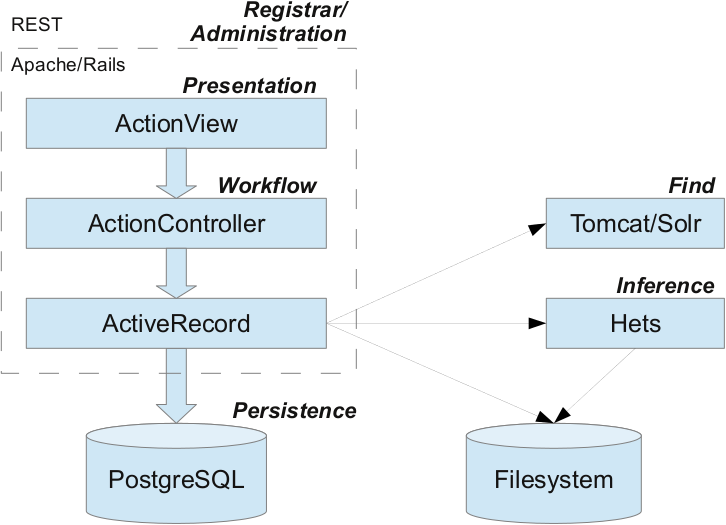
\includegraphics[width=0.8\textwidth]{architecture/ontohub-oor-architecture.png}
\end{frame}

\begin{frame}
\frametitle{Ontohub data model}
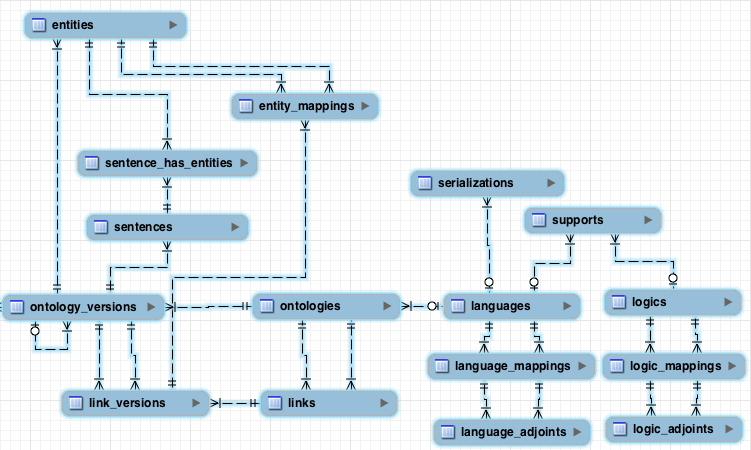
\includegraphics[width=\textwidth]{DBVisualization.png}
\end{frame}

\begin{frame}
\frametitle{OntoHub short-term and long-term goals}
\begin{itemize}
\item Documentation / rdoc / top-down overview
\item Keep functionality through tests
\item CRUD functionality not only for ontologies, but also for logics,
  translations, \ldots
\item display graph of ontologies and links (and logic graph)
\item Reasoning (provide Hets GUI)
\item Git backend (distributed development of ontologies)
\item long-term goal: OOR architecture
\end{itemize}
\end{frame}

\begin{frame}
\frametitle{Tests}
Test-driven development:\\
\emphc{No line of code without test}
\begin{itemize}
\item Fixtures: provide data for tests
\item Unit tests: test single methods of models
\item Functional tests: test controller actions
\item Integration tests: test sessions (sequences of actions)
\end{itemize}
\end{frame}

\begin{frame}
\frametitle{CRUD functionality for logics etc.}
\begin{itemize}
\item re-use existing functionality for ontologies
\item transfer this to links, logics, logic mappings,
languages,
language mappings, and
serializations
\item involve further tables like supports
\item display lists of these things: see display of graphs
\item read in logic graph from OntoIOp registry (RDF)
\end{itemize}
\end{frame}

\begin{frame}
\frametitle{OntoIOp registry}
\vspace{-1cm}
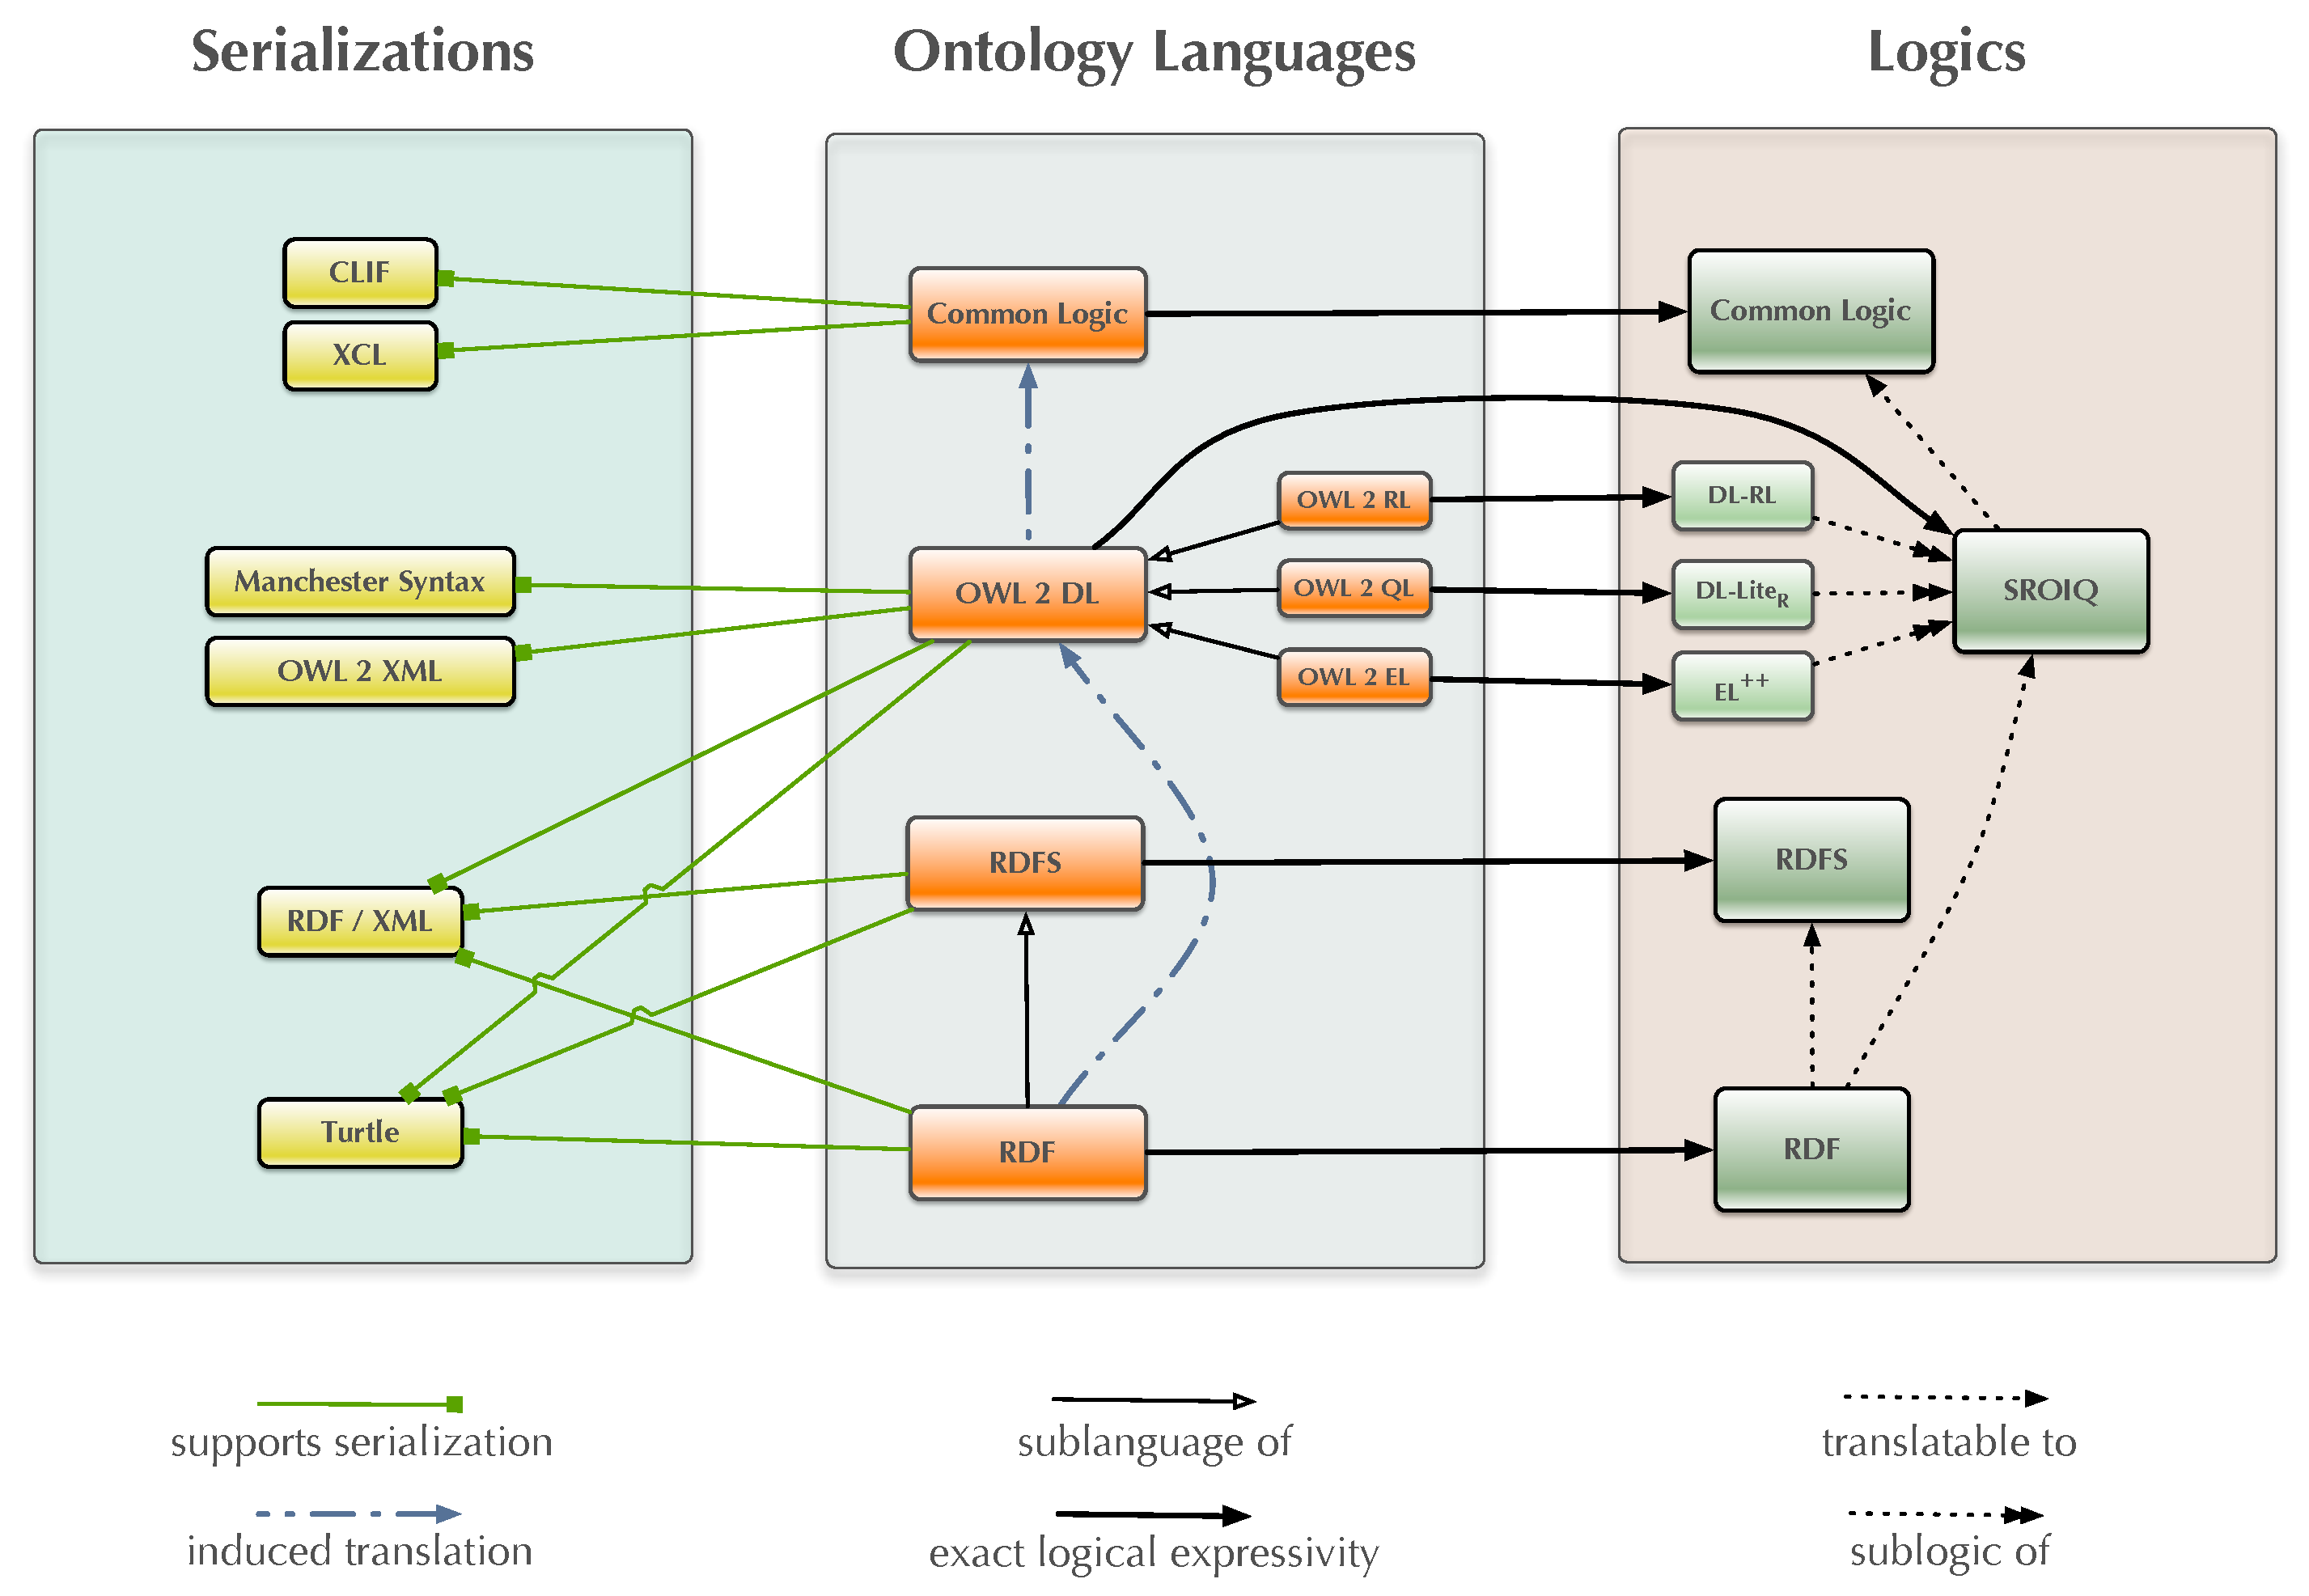
\includegraphics[width=0.9\textwidth]{DOL-ontograph-layers-TKE.pdf}
\end{frame}

\begin{frame}
\frametitle{display of graphs}
\begin{itemize}
\item use graphviz / dot to generate svg from graph
\item html and javascript can be embedded to svg
\item use this to realise menus for nodes and links
\item long-term goal: re-use Bioportal's fancy display
\end{itemize}
\end{frame}


\begin{frame}
\frametitle{OOR architecture}
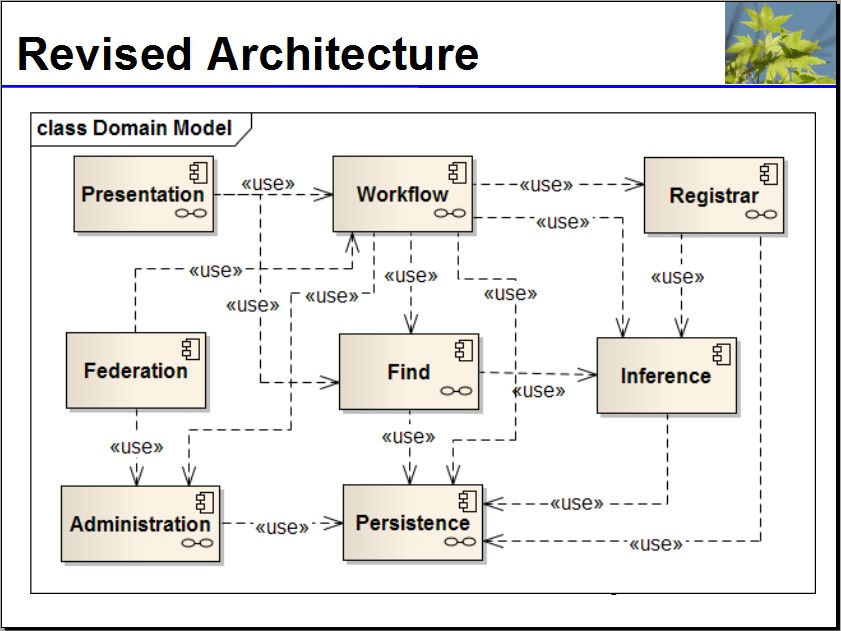
\includegraphics[width=\textwidth]{revised-OOR-architecture-proposal--ToddSchneider-KenBaclawski_20101119.jpg}
\end{frame}


\begin{frame}
\frametitle{Git backend}
\begin{itemize}
\item New Rails model ``repository'', which simultaneously provides namespace for ontologies
\item underlying git or svn repositories
\item permissions per repository (not per ontology)
\item only contents of master branch is displayed in Ontohub
\item store who has pushed when what
\item server side git hooks
\end{itemize}
\end{frame}

\begin{frame}
\frametitle{Organisation}
\begin{itemize}
\item who does what?
\item meetings
\item shared office in Cartesium
\end{itemize}
\end{frame}

\end{document}



Zielskizzen



Speichern: Wer hat was wann wohin gepusht?
server side hooks
http://git-scm.com/book/en/Customizing-Git-Git-Hooks#Server-Side-Hooks
Suche?
Evtl. NoSQL (MongoDB, CouchDB)



\begin{frame}
\frametitle{}
\begin{itemize}
\item 
\item 
\item 
\end{itemize}
\end{frame}
 	
